\section{Deelvraag 2: Architectuur}
In deze paragraaf zijn de resultaten voor deelvraag 2 \textit{\SubquestionTwo} verzameld en onderzocht.
Er is samen met de architect van het CMS Erwin Keuning (ook wel de schepper genoemd) en met Software engineer Kevin Snijder een IT archtecture sketching sessie gedaan.
Samen met Erwin en Kevin is het huidige systeem architectuur en data model besproken en in beeld gebracht, de afbeeldingen die gebruikt worden zijn afgeleid van de originele tekening die te vinden is in BIJLAGE X.
Verder is ook gebruik gemaakt van internere documentatie van het CMS, om de tekingen te onderstuenen.
\todo[inline]{Voeg bijlage toe aan bestand}
\subsection{Het Systeem}
Het eerste gedeelte van het IT Architecuture sketching is besteed aan het globale systeem / flow van het systeem.
Er zijn op dit moment 3 verschillende Snakeware Cloud site methodes deze methodes zijn XSL, Vue 2 en Vue 3 site.
De Vue 2 en 3 werken door middel van de Snakware Cloud API en de XSL werkt door middel van de Snakeware.Site code base.
In afbeelding \ref{fig:SystemArchitectureXSL} is te zien hoe de XSL sites werken, in afbeeldingen \ref{fig:SystemArchitectureVue} is te zien hoe de vue sites werken. 

\whitespace
\begin{graphic}
	\captionsetup{type=figure}
	\caption{Globale systeem architectuur}
	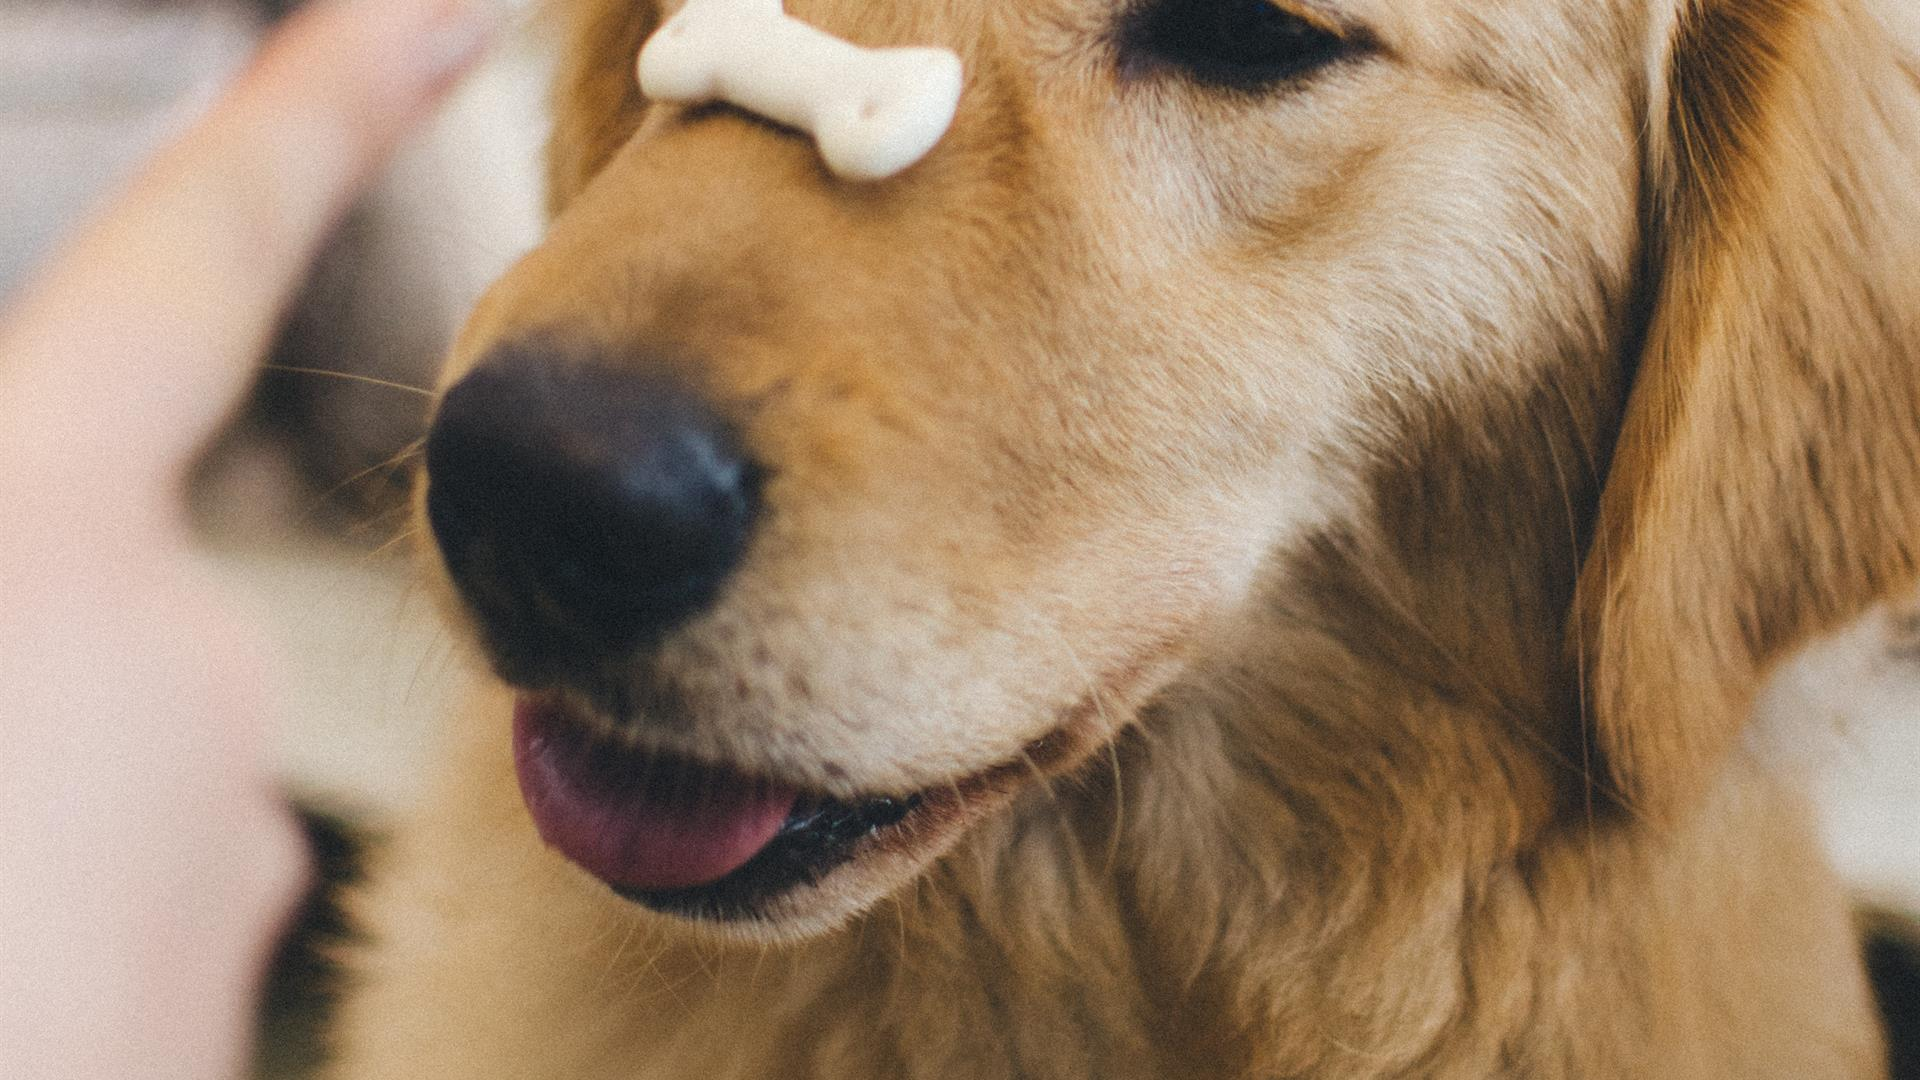
\includegraphics[scale=0.2]{Placeholder.jpg}
	\label{fig:SystemArchitectureXSL}
\end{graphic}

\whitespace
\begin{graphic}
    \captionsetup{type=figure}
    \caption{Globale systeem architectuur}
    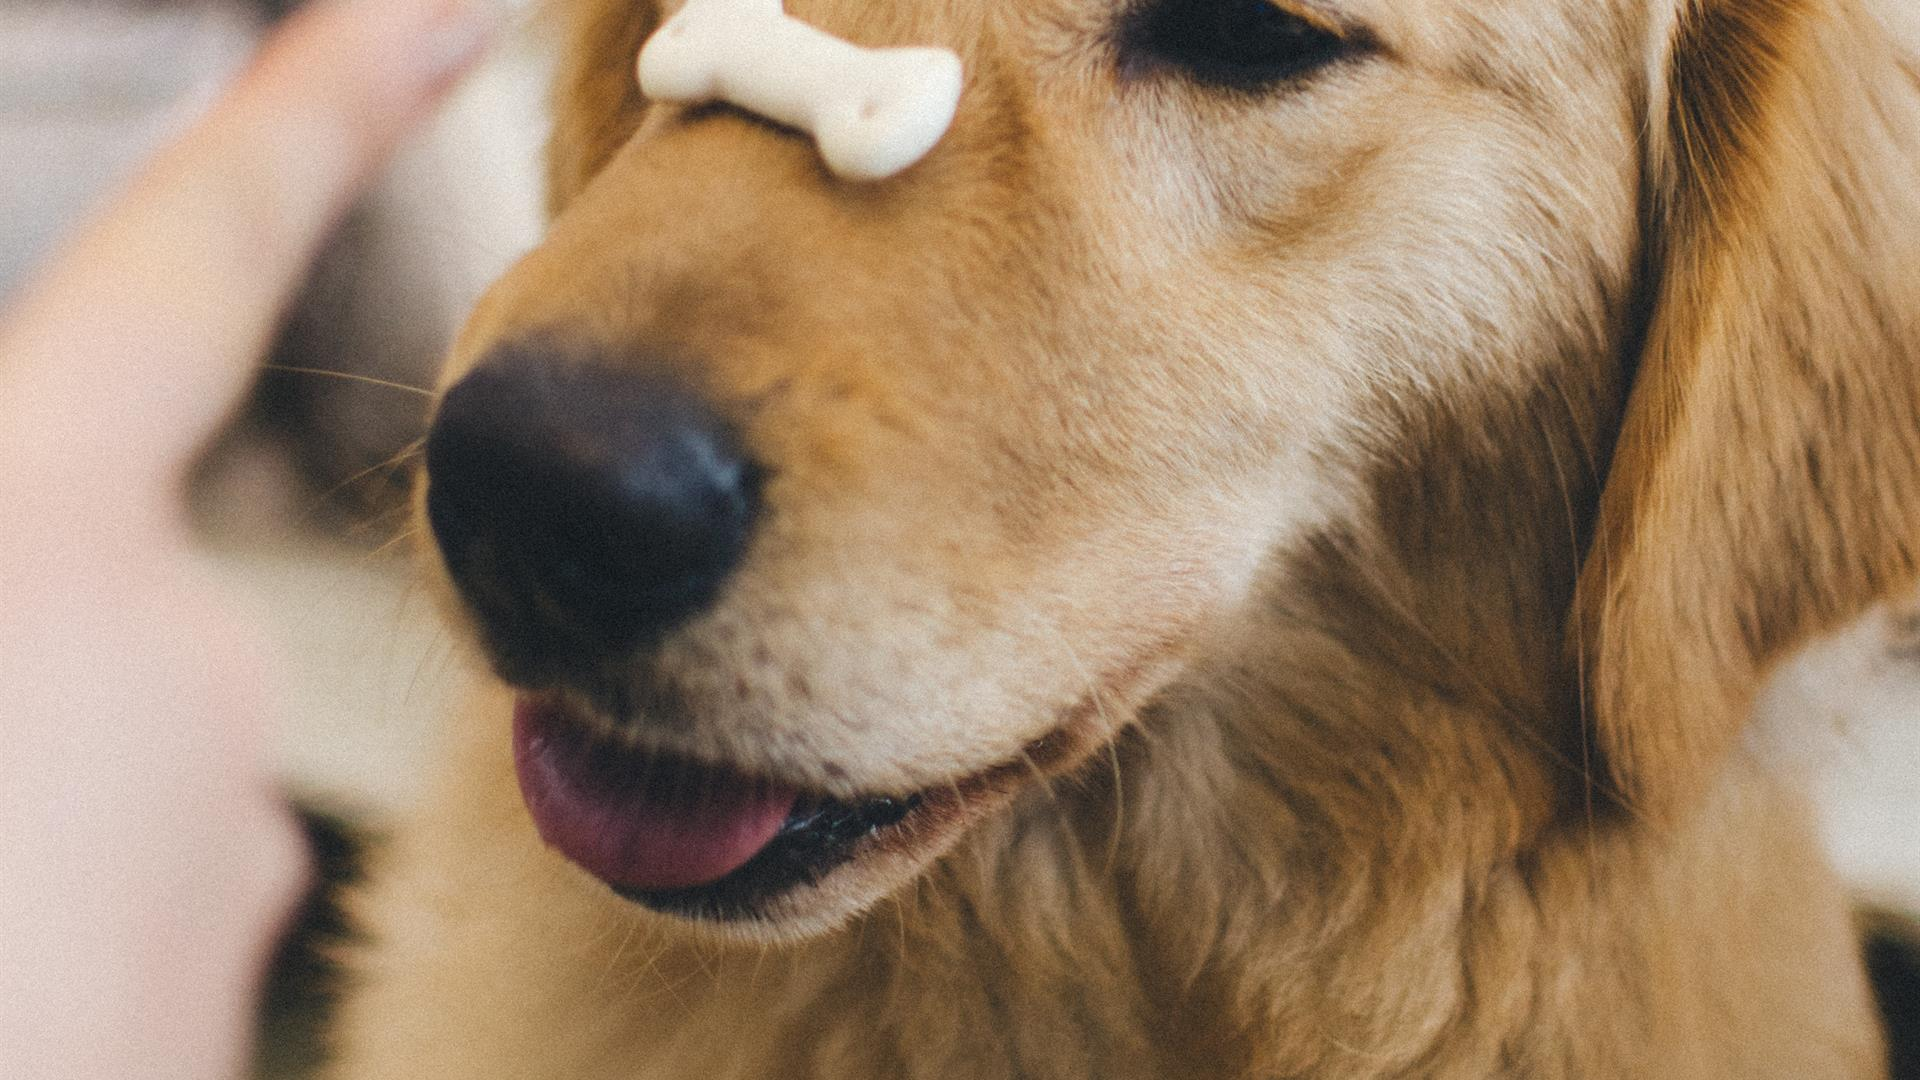
\includegraphics[scale=0.2]{Placeholder.jpg}
    \label{fig:SystemArchitectureVue}
\end{graphic}

Tijdens de IT Architeture sketching was er ook ruimte overgelaten om te onderzoeken waar er mogelijk verbeteringen gemaakt konden worden.
Een van de grote problemen nu met het huidige CMS is dat het niet gebruikt maakt van de SOLID prinicples (Personelijke cummunicatie erwin).
Ook is het CMS een grote Monolith dit zorgt er voor dat het niet goed schaalt met meerdere gebruikers.
Verder is het gebruik van XML ook niet optimaal meer dit is niet de snelste Data tranfer model en kan verbeterd worden.

\todo[inline]{Verbeter de teksten}
\todo[inline]{Opzoeken hoe je persoonlijke communicatie refereerd}

\subsection{Het Datamodel}
ook heel wow
